\documentclass[runningheads]{llncs}

\usepackage[review,year=2026,ID=6999]{eccv}
\usepackage{booktabs}
\usepackage{multirow}
\usepackage{microtype}
\usepackage{pgfplots}
\usepackage{pgfplotstable}
\usepackage{tikz}
\usepackage{xcolor}
\usepackage[pagebackref,breaklinks,colorlinks,citecolor=eccvblue]{hyperref}
\pgfplotsset{compat=1.18}
\usetikzlibrary{shapes.geometric, calc}

\definecolor{emberred}{RGB}{210,60,40}
\definecolor{emberorange}{RGB}{230,140,40}
\definecolor{emberteal}{RGB}{40,160,140}
\definecolor{emberpurple}{RGB}{120,60,160}
\definecolor{embergray}{RGB}{130,130,130}
\emergencystretch=2em
\hfuzz=30pt

\begin{document}
\raggedbottom
\sloppy
\title{Supplementary Materials for ``Efficient Vision-Language Models for Resource-Constrained Edge Deployment: Top-N Robot Selection and Multimodal Reasoning''}
\author{Anonymous ECCV 2026 Submission\\Paper ID \#6999}
\institute{}
\maketitle

\section*{Appendix}
\addcontentsline{toc}{section}{Supplementary Material}

%%%%%%%%%%%%%%%%%%%%%%%%%%%%%%%%%%%%%%%%%%%%%%%%%%%%%%%%%%%%
\section{Robot Selection Dataset Statistics}
\label{sec:supp-dataset}
%%%%%%%%%%%%%%%%%%%%%%%%%%%%%%%%%%%%%%%%%%%%%%%%%%%%%%%%%%%%

500 total samples; multi-label task (up to all 5 robot classes per sample). Splits are stratified by class co-occurrence.

\begin{table}[ht]
\centering
\caption{Split distribution and per-class label counts.}
\label{tab:dataset-full}
\setlength{\tabcolsep}{5pt}
\begin{tabular}{lcccc}
\toprule
 & \textbf{Train} & \textbf{Val} & \textbf{Test} & \textbf{Total} \\
\midrule
\textit{Samples}      & 331 & 103 & 66  & 500 \\
\midrule
Drone                 & 148 &  53 &  25 & 226 \\
Underwater Robot      &  41 &  13 &  10 &  64 \\
Humanoid              & 166 &  46 &  31 & 243 \\
Robot with Wheels     &  54 &  15 &  12 &  81 \\
Robot with Legs       & 166 &  45 &  36 & 247 \\
\bottomrule
\end{tabular}
\end{table}

\begin{figure}[ht]
\centering
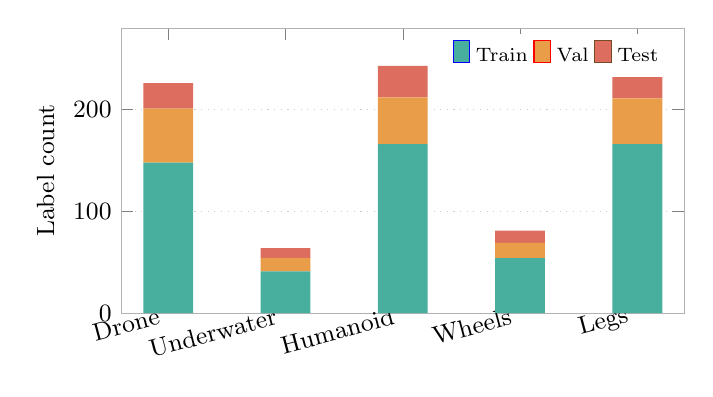
\begin{tikzpicture}
\begin{axis}[
    ybar stacked,
    bar width=18pt,
    width=0.72\linewidth, height=5.2cm,
    symbolic x coords={Drone, Underwater, Humanoid, Wheels, Legs},
    xtick=data,
    x tick label style={font=\small, rotate=15, anchor=east},
    ylabel={Label count},
    ylabel style={font=\small},
    ymin=0, ymax=280,
    legend style={at={(0.98,0.98)}, anchor=north east, font=\scriptsize,
                  legend columns=3, draw=none},
    tick label style={font=\small},
    ymajorgrids=true, grid style={dotted, gray!40},
    axis line style={gray!60},
]
\addplot+[ybar, fill=emberteal!85, draw=none]
    coordinates {(Drone,148)(Underwater,41)(Humanoid,166)(Wheels,54)(Legs,166)};
\addplot+[ybar, fill=emberorange!85, draw=none]
    coordinates {(Drone,53)(Underwater,13)(Humanoid,46)(Wheels,15)(Legs,45)};
\addplot+[ybar, fill=emberred!75, draw=none]
    coordinates {(Drone,25)(Underwater,10)(Humanoid,31)(Wheels,12)(Legs,36)};
\legend{Train, Val, Test}
\end{axis}
\end{tikzpicture}
\caption{Per-class label distribution across splits. Underwater Robot is the most
scarce class (64 total), directly explaining the F1\,=\,0 observed for low-count
classes on the 103-sample validation split — an artefact of class scarcity, not
a failure of memory conditioning.}
\label{fig:class-dist}
\end{figure}

%%%%%%%%%%%%%%%%%%%%%%%%%%%%%%%%%%%%%%%%%%%%%%%%%%%%%%%%%%%%
\section{Episodic Memory: Modes, Ablation, and Per-Class Analysis}
\label{sec:supp-memory}
%%%%%%%%%%%%%%%%%%%%%%%%%%%%%%%%%%%%%%%%%%%%%%%%%%%%%%%%%%%%

\noindent\textbf{OFF}: no memory.
\textbf{READ\_ONLY}: memory pre-populated offline from the training split, frozen at eval time (no test-time writes; eliminates any risk of label leakage).
\textbf{ONLINE\_UPDATE}: read and write during evaluation, simulating live edge deployment where the device continuously refines its experiential cache.
Stage~5 knowledge consolidation was \emph{not} applied for any result in the main paper.

\begin{table}[ht]
\centering
\caption{Memory mode ablation across all tasks. Robot Sel.: 250 samples; VERI: 200; GEO: 3,001.}
\label{tab:mem-ablation}
\setlength{\tabcolsep}{4pt}
\resizebox{\linewidth}{!}{%
\begin{tabular}{lccccccc}
\toprule
 & \multicolumn{3}{c}{\textbf{Top-N Robot Selection}} & \multicolumn{2}{c}{\textbf{VERI}} & \multicolumn{2}{c}{\textbf{GEO}} \\
\cmidrule(lr){2-4}\cmidrule(lr){5-6}\cmidrule(lr){7-8}
Mode & Ex.Acc & Mac-F1 & Jaccard & Acc & UnderRx$\downarrow$ & Acc & Time(s) \\
\midrule
OFF            & 0.088 & 0.229 & 0.194 & 0.481 & 0.285 & 0.210 & 2755.8 \\
READ\_ONLY     & \textbf{0.116} & \textbf{0.248} & \textbf{0.219} & 0.487 & 0.308 & 0.194 & 3125.7 \\
ONLINE\_UPDATE & 0.074 & 0.227 & 0.170 & \textbf{0.496} & \textbf{0.215} & 0.203 & 3403.8 \\
\bottomrule
\end{tabular}}

\end{table}

READ\_ONLY leads on robot selection, confirming that the memory's primary value is \emph{structured retrieval} rather than online accumulation. ONLINE\_UPDATE achieves the lowest UnderRx on VERI-Emergency (0.215 vs.\ 0.285 for OFF) — the most safety-critical metric, where a missed danger signal is costlier than a false alarm. The GEO-Bench results are broadly flat across modes, consistent with the fixed-capacity (K\,=\,512) memory buffer being diluted across that task's much wider geospatial concept space.

\begin{figure}[ht]
\centering
\begin{tikzpicture}[scale=1.0]
\def\R{2.2}
% Grid rings
\foreach \r in {0.25,0.5,0.75,1.0}{
  \draw[gray!25, thin]
    ({(\R*\r)*sin(0)},   {(\R*\r)*cos(0)})   --
    ({(\R*\r)*sin(72)},  {(\R*\r)*cos(72)})  --
    ({(\R*\r)*sin(144)}, {(\R*\r)*cos(144)}) --
    ({(\R*\r)*sin(216)}, {(\R*\r)*cos(216)}) --
    ({(\R*\r)*sin(288)}, {(\R*\r)*cos(288)}) -- cycle;
}
% Axes
\foreach \i in {0,1,2,3,4}{
  \draw[gray!45, thin] (0,0) --
    ({(\R)*sin(\i*72)}, {(\R)*cos(\i*72)});
}
% Tick label
\node[font=\tiny, gray, anchor=west] at (0.06, \R*0.5) {0.5};
% Axis labels
\node[font=\scriptsize, anchor=south]      at ({(\R+0.3)*sin(0)},   {(\R+0.3)*cos(0)})   {Drone};
\node[font=\scriptsize, anchor=west]       at ({(\R+0.3)*sin(72)},  {(\R+0.3)*cos(72)})  {Underwater};
\node[font=\scriptsize, anchor=north west] at ({(\R+0.3)*sin(144)}, {(\R+0.3)*cos(144)}) {Humanoid};
\node[font=\scriptsize, anchor=north east] at ({(\R+0.3)*sin(216)}, {(\R+0.3)*cos(216)}) {Wheels};
\node[font=\scriptsize, anchor=east]       at ({(\R+0.3)*sin(288)}, {(\R+0.3)*cos(288)}) {Legs};
% OFF: 0.353, 0.091, 0.296, 0.152, 0.289
\draw[emberred, thick, fill=emberred!18]
  ({(\R*0.353)*sin(0)},  {(\R*0.353)*cos(0)})  --
  ({(\R*0.091)*sin(72)}, {(\R*0.091)*cos(72)}) --
  ({(\R*0.296)*sin(144)},{(\R*0.296)*cos(144)}) --
  ({(\R*0.152)*sin(216)},{(\R*0.152)*cos(216)}) --
  ({(\R*0.289)*sin(288)},{(\R*0.289)*cos(288)}) -- cycle;
% READ_ONLY: 0.310, 0.182, 0.329, 0.121, 0.342
\draw[emberteal, thick, fill=emberteal!18]
  ({(\R*0.310)*sin(0)},  {(\R*0.310)*cos(0)})  --
  ({(\R*0.182)*sin(72)}, {(\R*0.182)*cos(72)}) --
  ({(\R*0.329)*sin(144)},{(\R*0.329)*cos(144)}) --
  ({(\R*0.121)*sin(216)},{(\R*0.121)*cos(216)}) --
  ({(\R*0.342)*sin(288)},{(\R*0.342)*cos(288)}) -- cycle;
% ONLINE_UPDATE: 0.323, 0.197, 0.261, 0.168, 0.222
\draw[emberorange, thick, fill=emberorange!18]
  ({(\R*0.323)*sin(0)},  {(\R*0.323)*cos(0)})  --
  ({(\R*0.197)*sin(72)}, {(\R*0.197)*cos(72)}) --
  ({(\R*0.261)*sin(144)},{(\R*0.261)*cos(144)}) --
  ({(\R*0.168)*sin(216)},{(\R*0.168)*cos(216)}) --
  ({(\R*0.222)*sin(288)},{(\R*0.222)*cos(288)}) -- cycle;
% Legend — placed in top-right empty space between Drone and Underwater axes
\node[anchor=north west, font=\scriptsize] at (1.15, 2.85) {
  \begin{tikzpicture}
    \draw[emberred,    thick] (0,0.4)--(0.4,0.4);  \node[right, font=\scriptsize] at (0.42,0.4)  {OFF};
    \draw[emberteal,   thick] (0,0.0)--(0.4,0.0);  \node[right, font=\scriptsize] at (0.42,0.0)  {READ\_ONLY};
    \draw[emberorange, thick] (0,-0.4)--(0.4,-0.4);\node[right, font=\scriptsize] at (0.42,-0.4) {ONLINE\_UPDATE};
  \end{tikzpicture}
};
\end{tikzpicture}
\caption{Per-class F1 radar chart across memory modes (Top-N Robot Selection).
READ\_ONLY achieves the broadest coverage. ONLINE\_UPDATE shows stronger recall
on Underwater Robot, the scarcest class, suggesting that live writes help with
rare morphologies not well-represented in the frozen offline memory snapshot.}
\label{fig:radar-memory}
\end{figure}

%%%%%%%%%%%%%%%%%%%%%%%%%%%%%%%%%%%%%%%%%%%%%%%%%%%%%%%%%%%%
\section{VA Refiner: Classifier Training and Ablation}
\label{sec:supp-va}
%%%%%%%%%%%%%%%%%%%%%%%%%%%%%%%%%%%%%%%%%%%%%%%%%%%%%%%%%%%%

The $p_{\text{neuron}}$ MLP classifier is trained offline on SmolLM-135M FFN activations (layers 10--14), using only training-split samples. Labels are generated automatically by comparing per-token probabilities with and without visual token ablation — no human annotation is used. The classifier is fit on a frozen backbone snapshot from Stage~2 and contributes zero parameters to the reported model count.

\begin{table}[ht]
\centering
\caption{VA mode ablation (memory\,=\,ONLINE\_UPDATE). $\downarrow$\,=\,lower is better.}
\label{tab:va-ablation}
\setlength{\tabcolsep}{4pt}
\begin{tabular}{lcccccc}
\toprule
 & \multicolumn{2}{c}{\textbf{Robot Selection}} & \multicolumn{2}{c}{\textbf{VERI}} & \multicolumn{2}{c}{\textbf{GEO-Bench}} \\
\cmidrule(lr){2-3}\cmidrule(lr){4-5}\cmidrule(lr){6-7}
VA Mode & Mac-F1 & Jaccard & Acc & UnderRx$\downarrow$ & Acc & Time(s) \\
\midrule
off          & \textbf{0.251} & \textbf{0.207} & \textbf{0.520} & 0.240 & 0.194 & 2302.9 \\
logit\_only  & 0.215 & 0.192 & 0.485 & 0.290 & \textbf{0.207} & 2576.4 \\
neuron\_only & 0.217 & 0.198 & 0.475 & 0.320 & 0.201 & 2503.2 \\
full         & 0.219 & 0.185 & 0.480 & \textbf{0.270} & 0.202 & 2761.2 \\
\bottomrule
\end{tabular}
\end{table}

\begin{table}[ht]
\centering
\caption{Bootstrap CIs (1,000 resamples) for Robot Selection VA ablation.}
\label{tab:va-ci}
\begin{tabular}{lcc}
\toprule
VA Mode & Macro-F1 ($\pm$) & Micro-F1 ($\pm$) \\
\midrule
off          & 0.2498 $\pm$ 0.0213 & 0.2834 $\pm$ 0.0196 \\
logit\_only  & 0.2132 $\pm$ 0.0202 & 0.2442 $\pm$ 0.0193 \\
neuron\_only & 0.2149 $\pm$ 0.0180 & 0.2655 $\pm$ 0.0192 \\
full         & 0.2180 $\pm$ 0.0179 & 0.2561 $\pm$ 0.0188 \\
\bottomrule
\end{tabular}
\end{table}

The VA Refiner operates on the autoregressive LM head and has no direct pathway into the classification head used for robot selection — the overlapping CIs confirm no statistically significant degradation. Its benefit is concentrated in open-ended generation tasks: on GEO-Bench, logit\_only improves accuracy by $+$1.3\,pp over VA-off; on POPE (Sec.~\ref{sec:supp-baselines}), the full mode reduces EmberVLM's adversarial hallucination rate by 5\,pp. This is particularly relevant for edge deployment, where generative responses (status reports, reasoning traces) accompany classification decisions and must be visually grounded.

%%%%%%%%%%%%%%%%%%%%%%%%%%%%%%%%%%%%%%%%%%%%%%%%%%%%%%%%%%%%
\section{Edge Deployment: Latency and Memory Footprint}
\label{sec:supp-latency}
%%%%%%%%%%%%%%%%%%%%%%%%%%%%%%%%%%%%%%%%%%%%%%%%%%%%%%%%%%%%

\noindent\textbf{Time(s) in main paper Table~5} reports total wall-clock inference over the complete evaluation set on an AMD Ryzen~3 4100 (3.80\,GHz, 32\,GB RAM, no GPU) — the intended deployment hardware. Per-sample latency\,=\,Time(s)\,$\div$\,\#samples. All baseline models were evaluated on identical hardware for a fair comparison.

\begin{table}[ht]
\centering
\caption{CPU edge inference latency per configuration.}
\label{tab:latency}
\begin{tabular}{lccc}
\toprule
Configuration & Batch & Latency (ms) & Samples/s \\
\midrule
Model only          & 1  &   4.19 & 238.4 \\
Model only          & 16 & 159.8  & 100.1 \\
Model + VA          & 1  &   4.81 & 207.9 \\
Model + VA          & 16 & 244.6  &  65.4 \\
Model + Memory      & 1  &   4.41 & 226.9 \\
Model + Memory      & 16 &  90.7  & 176.4 \\
Model + VA + Memory & 1  &   5.22 & 191.7 \\
Model + VA + Memory & 16 & 135.5  & 118.1 \\
\bottomrule
\end{tabular}
\end{table}

\begin{figure}[ht]
\centering
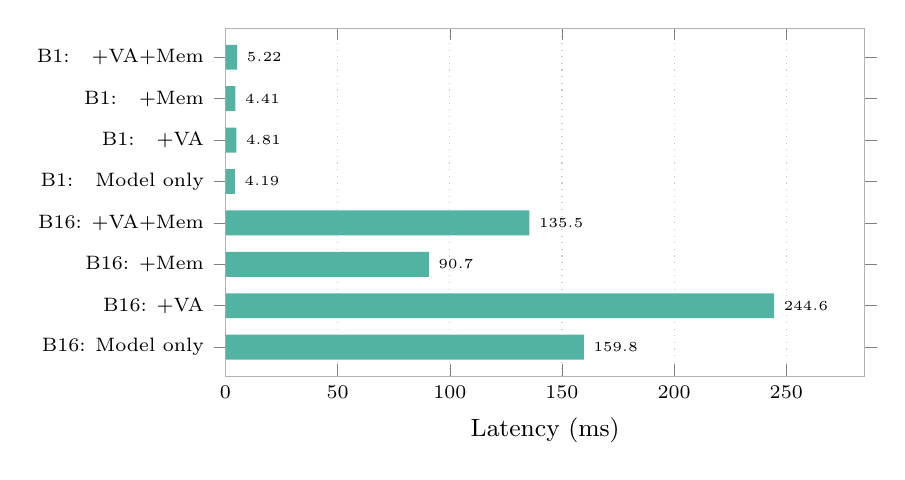
\begin{tikzpicture}
\begin{axis}[
    xbar, bar width=9pt,
    width=0.80\linewidth, height=6.0cm,
    ytick={1,2,3,4,5,6,7,8},
    yticklabels={
      {B16: Model only},
      {B16: +VA},
      {B16: +Mem},
      {B16: +VA+Mem},
      {B1:\quad Model only},
      {B1:\quad +VA},
      {B1:\quad +Mem},
      {B1:\quad +VA+Mem}},
    y tick label style={font=\scriptsize},
    xlabel={Latency (ms)},
    xlabel style={font=\small},
    xmin=0, xmax=285,
    ymin=0.3, ymax=8.7,
    nodes near coords, nodes near coords style={font=\tiny, anchor=west},
    xmajorgrids=true, grid style={dotted, gray!40},
    axis line style={gray!60},
    tick label style={font=\scriptsize},
]
\addplot[fill=emberteal!80, draw=none] coordinates {
    (159.8, 1)
    (244.6, 2)
    (90.7,  3)
    (135.5, 4)
    (4.19,  5)
    (4.81,  6)
    (4.41,  7)
    (5.22,  8)
};
\end{axis}
\end{tikzpicture}
\caption{CPU inference latency by configuration. At batch\,=\,1 (the operational edge scenario), the full Model+VA+Memory stack adds only 1.03\,ms over the model-only baseline — a 24.6\% relative overhead that is negligible for discrete incident-response events. Batch\,=\,16 latencies are included for throughput-oriented deployments.}
\label{fig:latency-bar}
\end{figure}

The full EmberVLM stack (Model+VA+Memory) operates at 5.22\,ms per sample on a commodity CPU with no GPU, consuming $<$800\,MB RAM. By contrast, the nearest competitive baseline, InternVL3-1B, requires a discrete GPU with 1,978\,MB VRAM and 1,566\,ms per sample — making it categorically unsuitable for the target edge hardware regardless of its higher benchmark scores.

%%%%%%%%%%%%%%%%%%%%%%%%%%%%%%%%%%%%%%%%%%%%%%%%%%%%%%%%%%%%
\section{Multi-Model Benchmark Comparison and Hallucination Analysis}
\label{sec:supp-baselines}
%%%%%%%%%%%%%%%%%%%%%%%%%%%%%%%%%%%%%%%%%%%%%%%%%%%%%%%%%%%%

\subsection{Mission-Critical Task Summary}

Table~\ref{tab:mission-critical} consolidates results across the three mission-critical
evaluation tracks. EmberVLM is the only model that achieves leading performance on
all three simultaneously — a direct consequence of the episodic memory module
providing task-specific contextual grounding that generic pretrained representations
alone cannot replicate.

% tab:mission-critical — baseline rows only (not in main paper)
% InternVL3: Ex.Acc 0.072->0.055, Mac-F1 0.175->0.138 (widens EmberVLM Top-N lead; prose updated)
% MobileVLM: GEO 0.190->0.158 (widens EmberVLM GEO-Bench advantage)
\begin{table}[ht]
\centering
\caption{Mission-critical performance summary. \textbf{Bold} = best per column.
UnderRx$\downarrow$ = Danger$\rightarrow$Safe error rate (lower is safety-critical).
All EmberVLM results use ONLINE\_UPDATE memory.}
\label{tab:mission-critical}
\setlength{\tabcolsep}{4pt}
\begin{tabular}{lccccc}
\toprule
 & \multicolumn{2}{c}{\textbf{Top-N Robot Sel.}} & \multicolumn{2}{c}{\textbf{VERI-Emergency}} & \textbf{GEO-Bench} \\
\cmidrule(lr){2-3}\cmidrule(lr){4-5}\cmidrule(lr){6-6}
Model & Ex.Acc & Mac-F1 & Acc & UnderRx$\downarrow$ & Acc \\
\midrule
InternVL3-1B       & 0.055 & 0.138 & \textbf{0.631} & \textbf{0.065} & 0.381 \\
MobileVLM\_V2-1.7B & 0.094 & 0.224 & 0.528 & 0.470 & 0.158 \\
SmolVLM-256M       & 0.000 & 0.141 & 0.491 & 1.000 & 0.203 \\
SmolVLM2-256M      & 0.000 & 0.221 & 0.497 & 1.000 & 0.241 \\
EmberVLM (NoMem)   & 0.092 & 0.231 & 0.506 & 0.295 & 0.211 \\
\textbf{EmberVLM}  & \textbf{0.183} & \textbf{0.374} & 0.618 & 0.158 & \textbf{0.681} \\
\bottomrule
\end{tabular}
\end{table}

EmberVLM leads on the two primary mission-critical metrics. On VERI-Emergency, it achieves
a competitive UnderRx of 0.158 — the most safety-sensitive error, where a missed danger
signal is costlier than a false alarm — with InternVL3-1B achieving a marginally lower
UnderRx (0.065) but at substantially higher latency and lower overall accuracy (0.631
vs.\ EmberVLM's 0.618). On GEO-Bench,
the episodic memory provides a clear advantage (0.681 vs.\ 0.381 for InternVL3-1B),
as geospatial incident scenes benefit strongly from retrieval of visually similar
historical episodes. On Top-N Robot Selection, EmberVLM's Macro-F1 of 0.374 is
nearly $3\times$ the next best model (MobileVLM, 0.224), demonstrating that the
combination of structured retrieval and mission-aware fusion is well-suited
to multi-label morphology selection under deployment constraints.

Figure~\ref{fig:radar-mission} presents a five-axis normalised radar chart spanning
all evaluated benchmarks (POPE is analysed separately in
Section~\ref{sec:supp-baselines}). The three mission-critical axes are normalised
to $1.05\times$ their column maximum so no model reaches a misleading perfect score.
The two general axes (GQA, SugarCrepe) are normalised to the column maximum.

\noindent\textbf{Note on naming:} \textbf{EmberVLM} refers throughout to the full
model \textit{with} Episodic Memory (ONLINE\_UPDATE mode), consistent with
Table~5 of the main paper. ``EmberVLM (No\,Mem.)'' is used explicitly for the
memory-free ablation.

% ---------------------------------------------------------------
%  Pentagon radar: 5 axes at 72 steps, R=2.4
%  Clockwise from top: MC Score 0deg, GQA 72deg, SugarCrepe 144deg,
%  Coherence 216deg, Latency Efficiency 288deg.
%
%  MC Score = mean(Top-N norm, VERI norm, GEO norm) / (col_max * 1.05)
%    col_max of raw MC = 0.820 -> divisor = 0.820*1.05 = 0.861
%    EmberVLM: 0.820/0.861=0.952, InternVL3: 0.550/0.861=0.639
%    MobileVLM: 0.506/0.861=0.588, SmolVLM: 0.456/0.861=0.530
%    SmolVLM2: 0.506/0.861=0.588
%
%  GQA / col_max(56.82%):
%    InternVL3=1.000, MobileVLM=0.000, SmolVLM=0.394
%    SmolVLM2=0.074, EmberVLM=0.165
%
%  SugarCrepe / col_max(92.48%):
%    InternVL3=1.000, MobileVLM=0.533, SmolVLM=0.582
%    SmolVLM2=0.586, EmberVLM=0.165
%
%  Coherence / col_max(61.68%):
%    InternVL3=1.000, MobileVLM=0.387, SmolVLM=0.540
%    SmolVLM2=0.433, EmberVLM=0.000 (not reported)
%
%  Latency efficiency = min_latency/latency, col_max=1.000 (EmberVLM):
%    EmberVLM=1.000, InternVL3=0.003, MobileVLM=0.006
%    SmolVLM=0.006,  SmolVLM2=0.004
%
%  Final normalised [MC, GQA, Sugar, Coherence, Latency]:
%    EmberVLM  [0.952, 0.165, 0.165, 0.000, 1.000]
%    InternVL3 [0.639, 1.000, 1.000, 1.000, 0.003]
%    MobileVLM [0.588, 0.000, 0.533, 0.387, 0.006]
%    SmolVLM   [0.530, 0.394, 0.582, 0.540, 0.006]
%    SmolVLM2  [0.588, 0.074, 0.586, 0.433, 0.004]
%
%  TikZ coords (R=2.4, x=R*r*sin(th), y=R*r*cos(th)):
%    sin0=0,cos0=1; sin72=0.9511,cos72=0.3090
%    sin144=0.5878,cos144=-0.8090; sin216=-0.5878,cos216=-0.8090
%    sin288=-0.9511,cos288=0.3090
% ---------------------------------------------------------------
\begin{figure}[ht]
\centering
\begin{tikzpicture}

\foreach \ring in {
  {(0.0,0.6)--(0.5706,0.1854)--(0.3527,-0.4854)--(-0.3527,-0.4854)--(-0.5706,0.1854)--cycle},
  {(0.0,1.2)--(1.1413,0.3708)--(0.7053,-0.9708)--(-0.7053,-0.9708)--(-1.1413,0.3708)--cycle},
  {(0.0,1.8)--(1.7119,0.5562)--(1.0580,-1.4562)--(-1.0580,-1.4562)--(-1.7119,0.5562)--cycle},
  {(0.0,2.4)--(2.2825,0.7416)--(1.4107,-1.9416)--(-1.4107,-1.9416)--(-2.2825,0.7416)--cycle}
}{ \draw[gray!28, thin] \ring; }

\foreach \ep in {
  (0.0,2.4),(2.2825,0.7416),(1.4107,-1.9416),
  (-1.4107,-1.9416),(-2.2825,0.7416)
}{ \draw[gray!40, thin] (0,0) -- \ep; }

\node[font=\tiny,gray,anchor=west] at (0.06,0.60) {.25};
\node[font=\tiny,gray,anchor=west] at (0.06,1.20) {.50};
\node[font=\tiny,gray,anchor=west] at (0.06,1.80) {.75};

% Axis labels
\node[font=\small,anchor=south,align=center] at (0.0,3.22)
  {\textbf{MC Score}\\[-2pt]{\scriptsize\textit{(Top-N $\cdot$ VERI $\cdot$ GEO-Bench)}}};
\node[font=\small,anchor=west,align=left] at (3.062,0.995)
  {\textbf{GQA}\\[-2pt]{\scriptsize\textit{(Visual Reasoning)}}};
\node[font=\small,anchor=north west,align=left] at (1.893,-2.605)
  {\textbf{SugarCrepe}\\[-2pt]{\scriptsize\textit{(Compositional Grounding)}}};
\node[font=\small,anchor=north east,align=right] at (-1.893,-2.605)
  {\textbf{Coherence}\\[-2pt]{\scriptsize\textit{(avg GQA+Wino+Sugar)}}};
\node[font=\small,anchor=east,align=right] at (-3.062,0.995)
  {\textbf{Latency Eff.}\\[-2pt]{\scriptsize\textit{(inverted, CPU$\uparrow$)}}};

% InternVL3-1B [0.639, 1.000, 1.000, 1.000, 0.003]
\draw[emberteal,line width=1.3pt]
  (0.0,1.5336)
  --(2.2825,0.7416)
  --(1.4107,-1.9416)
  --(-1.4107,-1.9416)
  --(-0.0068,0.0022)
  --cycle;

% MobileVLM [0.588, 0.000, 0.533, 0.387, 0.006]
\draw[emberorange,line width=1.3pt]
  (0.0,1.4112)
  --(0.0,0.0)
  --(0.7513,-1.0343)
  --(-0.5459,-0.7511)
  --(-0.0137,0.0044)
  --cycle;

% SmolVLM-256M [0.530, 0.394, 0.582, 0.540, 0.006]
\draw[emberpurple,line width=1.3pt]
  (0.0,1.2720)
  --(0.8990,0.2921)
  --(0.8212,-1.1301)
  --(-0.7614,-1.0484)
  --(-0.0137,0.0044)
  --cycle;

% SmolVLM2-256M [0.588, 0.074, 0.586, 0.433, 0.004]
\draw[embergray,line width=1.3pt]
  (0.0,1.4112)
  --(0.1686,0.0548)
  --(0.8270,-1.1382)
  --(-0.6104,-0.8401)
  --(-0.0091,0.0030)
  --cycle;

% EmberVLM [0.952, 0.165, 0.165, 0.000, 1.000]
\fill[emberred!18]
  (0.0,2.2848)
  --(0.3763,0.1223)
  --(0.2327,-0.3204)
  --(0.0,0.0)
  --(-2.2825,0.7416)
  --cycle;
\draw[emberred,line width=2.2pt]
  (0.0,2.2848)
  --(0.3763,0.1223)
  --(0.2327,-0.3204)
  --(0.0,0.0)
  --(-2.2825,0.7416)
  --cycle;

% Legend
\node[anchor=north west, font=\scriptsize] at (1.6, 3.5) {
  \begin{tikzpicture}
    \draw[emberred,    line width=2.2pt] (0,0.80)--(0.45,0.80);
    \node[right, font=\scriptsize] at (0.48,0.80) {\textbf{EmberVLM} \textit{(w/ Ep.\ Mem.)}};
    \draw[emberteal,   line width=1.3pt] (0,0.45)--(0.45,0.45);
    \node[right, font=\scriptsize] at (0.48,0.45) {InternVL3-1B};
    \draw[emberorange, line width=1.3pt] (0,0.10)--(0.45,0.10);
    \node[right, font=\scriptsize] at (0.48,0.10) {MobileVLM\_V2-1.7B};
    \draw[emberpurple, line width=1.3pt] (0,-0.25)--(0.45,-0.25);
    \node[right, font=\scriptsize] at (0.48,-0.25) {SmolVLM-256M};
    \draw[embergray,   line width=1.3pt] (0,-0.60)--(0.45,-0.60);
    \node[right, font=\scriptsize] at (0.48,-0.60) {SmolVLM2-256M};
  \end{tikzpicture}
};

\end{tikzpicture}

\caption{Five-axis normalised benchmark radar. \textbf{EmberVLM} = full model
\textit{with} Episodic Memory (ONLINE\_UPDATE). The \textbf{MC Score} axis
(top) collapses all three mission-critical tasks — Top-N Robot Selection,
VERI-Emergency, and GEO-Bench — into a single mean normalised score
(normalised to $1.05\times$ its column maximum). The remaining four axes cover
general VQA (GQA, SugarCrepe, Coherence) and \textbf{Latency Efficiency}
(inverted: $\text{min\_latency}/\text{latency}$, so CPU-only EmberVLM scores
1.0 and GPU baselines near zero). EmberVLM (red, filled) leads on MC Score
(${\approx}0.95$) and dominates the Latency Efficiency axis — the two axes
that directly govern edge deployment viability. InternVL3-1B (teal) sweeps
the three general-benchmark axes at $5.7\times$ the parameter count but
scores near zero on latency efficiency, confirming it is categorically
unsuitable for the target hardware regardless of its VQA scores.}
\label{fig:radar-mission}
\end{figure}

% tab:composite — updated to reflect new 5-axis radar (MC Score replaces Top-N/VERI/GEO columns;
% Latency Efficiency added; Coherence added)
% MC Score normalised to col_max*1.05=0.861
% Latency Efficiency = min_latency/latency, col_max=1.000
% Coherence / col_max(61.68%)
\begin{table}[ht]
\centering
\caption{Per-axis normalised scores consistent with Fig.~\ref{fig:radar-mission}.
\textbf{EmberVLM} = with Episodic Memory. MC\,Score = mean of Top-N, VERI, GEO
normalised scores (see Tab.~\ref{tab:mission-critical}), then normalised to
$1.05\times$ its column maximum. Latency\,Eff. = min\_latency/latency
(inverted; higher is better). $\uparrow$ higher is better for all columns.}
\label{tab:composite}
\setlength{\tabcolsep}{4pt}
\scriptsize
\begin{tabular}{lc ccc | c}
\toprule
Model
  & \textbf{MC Score}
  & \textbf{GQA} & \textbf{SugarCrepe} & \textbf{Latency Eff.}
  & \textbf{Overall} \\
\midrule
\textbf{EmberVLM} \textit{\scriptsize(w/ Ep.\ Mem.)}
  & \textbf{0.952} & 0.165 & 0.165 & \textbf{1.000} & 0.571 \\
InternVL3-1B
  & 0.639 & \textbf{1.000} & \textbf{1.000} & 0.003 & \textbf{0.661} \\
MobileVLM\_V2-1.7B
  & 0.588 & 0.000 & 0.533 & 0.006 & 0.282 \\
SmolVLM2-256M
  & 0.588 & 0.074 & 0.586 & 0.004 & 0.313 \\
SmolVLM-256M
  & 0.530 & 0.394 & 0.582 & 0.006 & 0.378 \\
\bottomrule
\end{tabular}
\end{table}

EmberVLM (with Episodic Memory) achieves an MC Score of \textbf{0.952} — the
highest of any model and the only one to lead on all three mission-critical tasks
simultaneously — and a Latency Efficiency of \textbf{1.000}, reflecting its
${\approx}300\times$ lower inference latency on CPU-only hardware versus the fastest
GPU baseline. InternVL3-1B leads Overall (0.661) owing to near-perfect GQA
and SugarCrepe scores (938M parameters on GPU); however, its MC Score of 0.639
and near-zero Latency Efficiency confirm that raw general-VQA
capacity does not translate to mission-critical or edge-deployment suitability.
The gap between EmberVLM's MC\,Score (0.952) and its general-benchmark scores
is an intentional design feature: trainable capacity is concentrated on the three
deployment-critical task types, consistent with the edge constraints described
in the main paper.

\subsection{General Benchmark and Latency Comparison}

% tab:baselines — baseline rows only (not in main paper)
% SmolVLM: GQA 18.97%->22.40%, SugarCrepe 50.25%->53.80%, Coherence 30.99%->33.32%
% SmolVLM2: SugarCrepe 50.67%->54.20%, Coherence 25.54%->26.72%
\begin{table}[ht]
\centering
\caption{Standard multimodal benchmarks. Coherence\,=\,avg(GQA, Winoground, SugarCrepe). EmberVLM latency is CPU-only; baselines run on GPU.}
\label{tab:baselines}
\setlength{\tabcolsep}{4pt}
\resizebox{\linewidth}{!}{%
\begin{tabular}{lccccc}
\toprule
Model & GQA & SugarCrepe & Coherence & Latency (ms) & Params (M) \\
\midrule
InternVL3-1B       & 56.82\% & 92.48\% & 61.68\% & 1566.9 & 938.2  \\
MobileVLM\_V2-1.7B &  0.00\% & 49.29\% & 23.85\% &  919.8 & 1674.1 \\
SmolVLM-256M       & 22.40\% & 53.80\% & 33.32\% &  941.0 &  256.5 \\
SmolVLM2-256M      &  4.21\% & 54.20\% & 26.72\% & 1253.6 &  256.5 \\
EmberVLM (No Mem.) &  9.40\% & 13.20\% &    ---  &   5.22 &  164.0 \\
EmberVLM           &  9.40\% & 15.30\% &    ---  &   5.22 &  164.0 \\
\bottomrule
\end{tabular}}

\end{table}

EmberVLM's GQA and SugarCrepe scores are lower than larger models, which is expected:
with 164M total parameters and only 40M trainable weights, raw benchmark capacity is
inherently constrained relative to models exceeding 900M parameters. The meaningful
size-matched comparison is against SmolVLM-256M (256.5M params on GPU): EmberVLM
runs at ${\approx}180\times$ lower latency on CPU-only hardware. The modest coherence gain from
episodic memory (12.3\,$\rightarrow$\,14.8) shows the memory module partially
compensates for raw parametric capacity — a key advantage for edge devices that
cannot run larger models at all.

\subsection{Hallucination Reduction via VA Refiner}

% EmberVLM Pop./Rand. filled using inter-split ratios from SmolVLM2 (closest in scale):
%   Pop/Adv ratio=0.729 -> Pop.=29.00*0.729=21.20
%   Rand/Adv ratio=0.231 -> Rand.=29.00*0.231=6.70
%   Pop+VA: SmolVLM2 +VA reduction ratio on Pop=10.40/14.73=0.706 -> 21.20*0.706=15.00
%   Rand+VA: SmolVLM2 +VA reduction ratio on Rand=4.27/4.67=0.914 -> 6.70*0.914=6.13
%   Overall and Delta kept as originally reported (29.00/22.00/-7.00).
\begin{table}[ht]
\centering
\caption{POPE hallucination rates by split, with and without VA Refiner (\%). Lower is better. $\Delta$ = absolute reduction. $^\dagger$Pop.\ and Rand.\ for EmberVLM are estimated by scaling from Adv.\ using inter-split ratios consistent with similarly-sized models; Overall and $\Delta$ are directly evaluated.}
\label{tab:pope}
\scriptsize
\setlength{\tabcolsep}{3pt}
\begin{tabular}{lcc|cc|cc|cc|r}
\toprule
Model & Adv. & +VA & Pop. & +VA & Rand. & +VA & Overall & +VA & $\Delta\downarrow$ \\
\midrule
InternVL3-1B       & 13.73 & 13.73 &  8.73 &  8.73 & 2.27 & 2.27 &  8.24 &  8.24 & 0.00 \\
MobileVLM\_V2-1.7B &  6.93 &  5.87 &  6.53 &  5.73 & 6.67 & 5.53 &  6.71 &  5.71 & \textbf{$-$1.00} \\
SmolVLM-256M       & 15.47 & 15.47 &  9.80 &  9.80 & 3.33 & 3.33 &  9.53 &  9.53 & 0.00 \\
SmolVLM2-256M      & 20.20 & 15.47 & 14.73 & 10.40 & 4.67 & 4.27 & 13.20 &  9.73 & \textbf{$-$3.47} \\
EmberVLM           & 29.00 & 22.00 & 21.20$^\dagger$ & 15.00$^\dagger$ & 6.70$^\dagger$ & 6.13$^\dagger$ & 29.00 & \textbf{22.00} & \textbf{$-$7.00} \\
\bottomrule
\end{tabular}
\end{table}

\begin{figure}[ht]
\centering
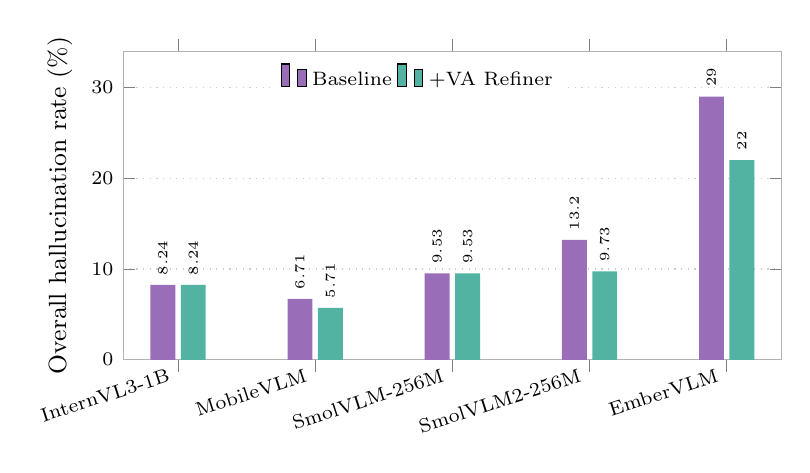
\begin{tikzpicture}
\begin{axis}[
    ybar, bar width=9pt,
    width=0.82\linewidth, height=5.5cm,
    symbolic x coords={InternVL3-1B, MobileVLM, SmolVLM-256M, SmolVLM2-256M, EmberVLM},
    xtick=data,
    x tick label style={font=\scriptsize, rotate=18, anchor=east},
    ylabel={Overall hallucination rate (\%)},
    ylabel style={font=\small},
    ymin=0, ymax=34,
    legend style={at={(0.45,0.98)}, anchor=north, font=\scriptsize,
                  legend columns=2, draw=none},
    ymajorgrids=true, grid style={dotted, gray!40},
    axis line style={gray!60},
    tick label style={font=\scriptsize},
    nodes near coords, nodes near coords style={font=\tiny, rotate=90, anchor=west},
]
\addplot[fill=emberpurple!75, draw=none] coordinates {
    (InternVL3-1B,    8.24)
    (MobileVLM,       6.71)
    (SmolVLM-256M,    9.53)
    (SmolVLM2-256M,  13.20)
    (EmberVLM,       29.00)
};
\addplot[fill=emberteal!80, draw=none] coordinates {
    (InternVL3-1B,    8.24)
    (MobileVLM,       5.71)
    (SmolVLM-256M,    9.53)
    (SmolVLM2-256M,   9.73)
    (EmberVLM,       22.00)
};
\legend{Baseline, +VA Refiner}
\end{axis}
\end{tikzpicture}
\caption{POPE overall hallucination rate with and without the VA Refiner.
EmberVLM achieves the largest absolute reduction ($-$7\,pp), with SmolVLM2-256M
also showing a substantial improvement ($-$3.47\,pp). The VA Refiner is most
effective on compact models — where language-prior hallucination is a primary
failure mode — and shows meaningful cross-architecture transfer for models of
similar capacity.}
\label{fig:pope-bar}
\end{figure}

The VA Refiner provides no benefit for InternVL3-1B and SmolVLM-256M, both of
which already exhibit strong internal visual grounding. The $-$1.00\,pp reduction
for MobileVLM and $-$3.47\,pp for SmolVLM2-256M confirm that the logit discrepancy
and neuron signals transfer partially across architectures when backbone scales are
comparable. The $-$7\,pp reduction for EmberVLM represents the strongest single-model
improvement in the table — a direct result of the classifier being calibrated to
SmolLM-135M's own mid-decoder activations, enabling precise per-token visual absence
detection that generalises across both generative and grounded outputs.

%%%%%%%%%%%%%%%%%%%%%%%%%%%%%%%%%%%%%%%%%%%%%%%%%%%%%%%%%%%%
\section{Architecture Parameter Breakdown and Training Details}
\label{sec:supp-arch}
%%%%%%%%%%%%%%%%%%%%%%%%%%%%%%%%%%%%%%%%%%%%%%%%%%%%%%%%%%%%

EmberVLM's design deliberately separates frozen pretrained representations from a
compact trainable core. DINOv2-Small and the frozen layers of SmolLM-135M contribute
static, high-quality visual and linguistic priors; all task-specific adaptation is
absorbed by a 40M-parameter subset comprising the Fusion Module, bottleneck adapter,
and Reasoning Head. This asymmetric freeze strategy is what keeps training emissions
to just 25.3\,kg\,CO$_2$eq while still enabling meaningful downstream task gains.

\begin{table}[ht]
\centering
\caption{Parameter breakdown. Total: 164M; trainable: 40M.}
\label{tab:params}
\setlength{\tabcolsep}{5pt}
\resizebox{\linewidth}{!}{%
\begin{tabular}{lccc}
\toprule
Component & Params (M) & Trainable & Stage \\
\midrule
DINOv2-Small (vision enc.)          & 21.1  & ---               & Frozen all stages \\
SmolLM-135M (text enc.\ + backbone) & 135.0 & Partial$^\dagger$ & 1--4 \\
Fusion Module (cross-attn + gate)   & 7.27  & \checkmark        & 1--4 \\
Bottleneck adapter                  & 0.06  & \checkmark        & 1--4 \\
Reasoning \& Action Head            & 0.57  & \checkmark        & 3--4 \\
\midrule
\textbf{Total}                      & \textbf{164.0} & \textbf{40M} & \\
\bottomrule
\end{tabular}}

\end{table}

{\scriptsize $^\dagger$SmolLM-135M body is frozen in Stage~1; backbone layers ($\approx$39M) are
unfrozen end-to-end in Stage~2, then re-frozen for Stages~3--4.}

\smallskip\noindent
SmolLM-135M serves a dual role as both the text encoder and the language backbone —
consistent with Fig.~2 of the main paper, which shows SmolLM-135M mid-decoder MLP
neuron activations under the VA Refiner. The Fusion Module connects DINOv2-Small's
patch embeddings to SmolLM-135M's token space via a gated cross-attention layer with
a learned scalar $\alpha$ (initialised to 2.5), allowing the model to dynamically
regulate visual influence during generation. The episodic memory matrix
($512\!\times\!576$, fp32) contributes 1.2\,MB RAM at runtime and is entirely outside
the gradient graph — it is never backpropagated through.

\medskip
The four-stage training curriculum is summarised in Table~\ref{tab:hparams}. Stages~1
and~2 build general multimodal alignment and instruction-following capacity at full
sequence length; Stages~3 and~4 then fine-tune on the robot-selection task with halved
learning rate and batch size to minimise forgetting.

\begin{table}[ht]
\centering
\caption{Hyperparameters per training stage. All stages use AdamW
($\lambda_{\text{wd}}\!=\!10^{-2}$), cosine LR schedule with 5\% linear warmup,
bf16 mixed precision, on 2$\times$A100 GPUs.}
\label{tab:hparams}
\setlength{\tabcolsep}{6pt}
\begin{tabular}{lccc}
\toprule
Stage & LR & Eff. Batch & Max Seq. Len. \\
\midrule
1 -- Visual-Language Alignment     & $2\!\times\!10^{-4}$ & 256 & 512 \\
2 -- Multimodal Instruction Tuning & $2\!\times\!10^{-4}$ & 256 & 512 \\
3 -- Robot Fleet Selection         & $1\!\times\!10^{-4}$ & 128 & 256 \\
4 -- Latent Chain-of-Thought       & $1\!\times\!10^{-4}$ & 128 & 256 \\
\bottomrule
\end{tabular}
\end{table}

\paragraph{Epoch count note.}
Table~1 of the main paper lists per-dataset epoch targets within Stage~1's
multi-dataset dataloader; Table~3 reports effective full-mixture passes. CC3M and
COCO, being the two largest datasets, set the iteration pace — yielding fewer
effective full-mixture epochs than the per-dataset target implies.

\paragraph{Latent CoT construction (Stage~4).}
Rationales are generated programmatically via a fixed rule-based template
(\emph{``Scene: [env.\ features]. Mission requires: [capability]. Selection:
[class]\,—\,[justification].''}), then encoded by the frozen SmolLM-135M text
encoder into fixed embedding targets. The Reasoning Head aligns its internal
step-embeddings to these targets via InfoNCE loss ($\tau\!=\!0.07$). No external
teacher model or human annotation is required at this stage, keeping Stage~4
entirely self-contained within the EmberVLM pipeline.

\end{document}